\documentclass[11pt,oneside]{article}
\usepackage[T1]{fontenc}
\usepackage[utf8]{inputenc}
\usepackage{lmodern}
\usepackage{microtype}
\usepackage{amsmath,amssymb,amsthm,mathtools}
\usepackage[a4paper,margin=1in]{geometry}
\usepackage{enumitem}
\usepackage{booktabs,longtable,array,tabularx}
\usepackage{tikz}
\usetikzlibrary{arrows.meta,positioning,calc,decorations.pathreplacing}
\usepackage{listings}
\usepackage{xcolor}
\usepackage{xurl}
\usepackage{fancyhdr}
\usepackage{needspace}
\usepackage{hyperref}
\usepackage{bookmark}
\usepackage[nameinlink,capitalise,noabbrev]{cleveref}

\hypersetup{
  colorlinks=true,
  linkcolor=blue!45!black,
  citecolor=green!35!black,
  urlcolor=blue!50!black,
  pdftitle={Certified Observation Towers: a general iPRA embedding framework with topology as a case study},
  pdfauthor={OpenAI, prepared for Vladimir Reshetnikov}
}

\pagestyle{fancy}
\fancyhf{}
\fancyhead[L]{Certified Observation Towers in iPRA}
\fancyhead[R]{\thepage}
\setlength{\headheight}{14pt}

\newtheorem{theorem}{Theorem}[section]
\newtheorem{lemma}[theorem]{Lemma}
\newtheorem{proposition}[theorem]{Proposition}
\newtheorem{corollary}[theorem]{Corollary}
\newtheorem{principle}[theorem]{Design principle}
\theoremstyle{definition}
\newtheorem{definition}[theorem]{Definition}
\newtheorem{example}[theorem]{Example}
\newtheorem{construction}[theorem]{Construction}
\theoremstyle{remark}
\newtheorem{remark}[theorem]{Remark}
\newtheorem{warning}[theorem]{Warning}

\newcommand{\N}{\mathbb{N}}
\newcommand{\Z}{\mathbb{Z}}
\newcommand{\Q}{\mathbb{Q}}
\newcommand{\R}{\mathbb{R}}
\newcommand{\Ftwo}{\mathbb{F}_{2}}
\newcommand{\ipra}{\ensuremath{\mathrm{iPRA}}}
\newcommand{\PRAAx}{\ensuremath{\mathsf{PRAAx}}}
\newcommand{\Prf}{\ensuremath{\mathsf{Prf}}}
\newcommand{\bits}{\ensuremath{\mathsf{Bits}}}
\newcommand{\carrier}{\ensuremath{\mathcal{C}}}
\newcommand{\obs}{\ensuremath{\mathsf{Obs}}}
\newcommand{\Simplex}{\ensuremath{\mathsf{Simplex}}}
\newcommand{\Valid}{\ensuremath{\mathsf{Valid}}}
\newcommand{\mesh}{\ensuremath{\mathsf{mesh}}}
\newcommand{\code}[1]{\texttt{#1}}
\newcommand{\Set}[1]{\left\{#1\right\}}
\newcommand{\angles}[1]{\left\langle #1\right\rangle}
\newcommand{\restr}{\mathord{\upharpoonright}}
\newcommand{\defeq}{\mathrel{:=}}
\newcommand{\powerset}{\mathcal{P}}
\newcommand{\todoformal}{\textsc{object-proof target}}

\lstdefinestyle{lean}{
  basicstyle=\ttfamily\small,
  columns=fullflexible,
  breaklines=true,
  frame=single,
  showstringspaces=false,
  keywordstyle=\bfseries,
  commentstyle=\itshape
}
\lstset{style=lean}

\title{\textbf{Certified Observation Towers}\\
A general framework for embedding mathematics into intuitionistic primitive recursive arithmetic, with topology as a case study}
\author{Prepared for Vladimir Reshetnikov}
\date{15 November 2026}

\begin{document}
\maketitle

\begin{abstract}
This report develops a reusable method for placing mathematical concepts and proofs inside intuitionistic primitive recursive arithmetic (\ipra).  The method begins with the current ProveIt infrastructure---fixed primitive-recursive symbols, bounded Boolean tests, quantifier-free induction, finite contracts, and the existing bridge from ordinary \ipra\ derivations to the concise native calculus---and adds a missing topological and choice-stable layer.

The central new organizing object is a \emph{certified observation tower}: an inverse tower of finite nerves whose refinement maps are represented not by arbitrary exact choices but by finite simplicial carriers.  A carrier assigns a nonempty cloud of possible target cells to every source cell.  Its strong simplex condition implies that every deterministic selection is simplicial, any two selections are contiguous, and their chain maps are related by an explicit finite prism homotopy.  Consequently homology maps are independent of boundary choices.  Carrier composition is finite relational composition, so continuous maps and their compositions can be represented without a discontinuous global selector.

The report gives complete human-readable proofs of the bounded Booleanization principle, finite-space/preorder equivalence, carrier composition, selection independence, the mod-2 prism identity, functorial homology for observation towers, and several closure constructions.  It explains how compactness, connectedness, separation, products, subspaces, quotients, homotopies, manifolds, fixed-point arguments, Jordan separation, and dimension obstruction should be stated as arithmetic schemas with explicit finite data and moduli.  It also identifies genuine boundaries: unrestricted quantification over open sets or functions is not first-order arithmetic, exact choice at collisions is not constructively free, and finite verification never manufactures a missing modulus, height bound, or exhaustion theorem.

The package includes an exact Python kernel and 15 passing tests for finite preorders, simplicial carriers, tower composition, mod-2 homology, and the prism identity.  It also includes two Lean blueprints: a semantic finite-topology layer and an object-language completion plan using the actual ProveIt declarations \code{PR}, \code{PTm}, \code{PRAAx}, \code{PRA.qfInd}, \code{Prf}, \code{NFm.ofPRA}, and \code{pra\_iff\_native}.  The Lean files are deliberately marked as uncompiled outlines; no unfinished semantic theorem is presented as an \ipra\ derivation.
\end{abstract}

\tableofcontents
\clearpage


\section{Repository audit and exact proof status}
\label{sec:audit}

\subsection{The arithmetic backend}

The relevant ProveIt development has a precise formal core.  In its ordinary presentation, \ipra\ has one function symbol for every primitive-recursive definition, the defining equations for those symbols, the successor axioms, intuitionistic first-order natural deduction with equality, and induction restricted to quantifier-free formulas.  The Lean types are \code{PR k} for a $k$-ary primitive-recursive symbol, \code{PTm n} for terms with $n$ free variables, \code{PRAAx} for the axiom family, and \code{Prf} for derivations.  The theorem \code{PRA.qfInd} is the actual induction endpoint.  The current library also proves
\[
  (\Gamma\vdash_{\PRAAx}\varphi)
  \quad\Longleftrightarrow\quad
  \mathsf{NPrf}(\mathsf{ofPRA}(\Gamma),\mathsf{ofPRA}(\varphi)),
\]
under the name \code{pra\_iff\_native}.  Thus the correct workflow is to construct an ordinary object-language derivation first and transport it only afterwards.  The bridge does not turn a true statement about natural numbers, or an ambient Lean theorem, into an \ipra\ derivation automatically \cite{ProveIt}.

This distinction is the main quality gate for the present report.  Every mathematical algorithm described below has three possible statuses:
\begin{enumerate}[label=(\roman*)]
  \item a human proof that a finite algorithm is correct;
  \item a semantic Lean theorem about that algorithm;
  \item an actual object-language term of type $\Gamma\vdash_{\PRAAx}\varphi$.
\end{enumerate}
Only (iii) is an internal \ipra\ proof.  The supplied Lean files specify a path from (i) to (iii), but do not claim to have completed it.

\subsection{What the existing proof packets already achieve}

The repository contains a large collection of delivered packets.  They establish a strong common style:
\begin{itemize}
  \item replace arbitrary real objects by fixed primitive-recursive evaluators, rational approximants, and explicit moduli;
  \item replace compactness by finite grids or finite nets;
  \item replace exact sign or branch tests by strict margins, overlap, or positive separation data;
  \item package algorithms as bounded traces with Boolean invariants;
  \item state explicitly that exact reference programs and semantic Lean lemmas do not by themselves constitute an object-language proof.
\end{itemize}

The strongest current foundational packet, ``finite contracts'', already gives compiled semantic lemmas, a copied and audited object kernel, actual object-\ipra\ examples, and a contract record that contains both a fixed \code{PR} program and a \code{Prf PRAAx} certificate.  Other packets contribute variable-length recursion, coherent finite presentations, relational outputs, backward demand analysis, and finite observation compilers.  These ingredients are not repeated here; they are reorganized into one topological calculus.

\subsection{The topology packets and their remaining gap}

Two existing topology packets are particularly important.

The dimension packet proves a finite rational theorem.  A table
$F:\{0,\ldots,N\}^{d}\to\Q^{m}$ whose opposite source faces stay $h$ apart, and whose image on every Kuhn simplex has diameter below $h/d$, must satisfy $d\leq m$.  The positive alternative extracts either a close opposite-face pair or a large same-simplex oscillation.  A cubical Sperner parity argument and staggered target grids drive the proof.  The passage to presented homeomorphisms uses fixed evaluators and explicit local uniform moduli.

The Jordan packet works with a circle embedding given by rational approximation routines, a forward continuity modulus, and a positive inverse-separation modulus.  It constructs a stable inside/outside bit only for points with positive clearance, uses finite crossing parity, and produces polygonal routes with certified clearance.  Crossing paths yield arbitrarily accurate approximate contacts; the packet does not silently assert an exact intersection parameter.

Both reports give substantial complete human arguments, but their Lean files are explicitly scaffolds.  Moreover, they solve theorem-specific finite combinatorics.  They do not yet supply a reusable answer to the following common question:

\begin{quote}
When a point, cell, root, chart, or branch lies on a finite boundary and several exact choices are compatible with all available observations, how can a map be composed and a topological invariant be proved independent of the choice, without invoking a discontinuous selector?
\end{quote}

The new ingredient of this report is a finite relational answer: retain the whole compatible cloud as a \emph{simplicial carrier}; prove that all selections are contiguous; and use an explicit prism homotopy to show choice independence on homology.  This is a classical topological mechanism in finite, proof-producing form.  It is closely related to the carrier methods of algebraic topology \cite{Munkres}, but the point here is its exact role as an \ipra\ interface.

\subsection{Audit conclusion}

The repository's recurring difficulties can be divided into three classes.

\begin{enumerate}[label=\textbf{A\arabic*.},leftmargin=2.5em]
  \item \textbf{Representation difficulties.}  Arbitrary functions, open sets, measures, or infinite structures are higher-type.  They must be replaced by fixed evaluators, finite observations, or explicit finite tables.
  \item \textbf{Constructive stability difficulties.}  Exact boundary choice, exact sign at zero, eigenvector selection at multiplicity, and branch selection at collision may be discontinuous.  They require overlap, a relational output, or an apartness gap.
  \item \textbf{Proof-internalization difficulties.}  A finite algorithm may be mathematically correct yet still lack Booleanization lemmas, defining-equation derivations, loop invariants, or the final $\Prf\ \PRAAx$ term.
\end{enumerate}

Certified observation towers address A1 and A2 uniformly for topology and many adjacent subjects.  The bounded proof compiler described in \cref{sec:contracts,sec:lean} addresses A3 at the level of a precise implementation plan.  The framework does not pretend that missing analytic moduli, Diophantine height bounds, or theorem-specific parity arguments can be obtained by encoding alone.


\section{Statement discipline: what an \ipra\ theorem may say}
\label{sec:discipline}

\subsection{First-order schemas rather than hidden higher types}

A first-order arithmetic theory quantifies over natural numbers.  It does not quantify directly over arbitrary functions $\N\to\N$, arbitrary subsets of a space, or arbitrary topological spaces.  There are three legitimate ways to express such data.

\begin{definition}[Fixed-symbol schema]
Choose a particular primitive-recursive evaluator $e$ and add its fixed \code{PR} syntax tree to the statement.  Prove the theorem uniformly in the numerical inputs to $e$, but not by quantifying over the set of all evaluator codes.
\end{definition}

\begin{definition}[Finite-table input]
For a requested precision $k$, pass a number coding exactly the finite table read by the proof.  A bounded verifier checks the table and the local compatibility laws.
\end{definition}

\begin{definition}[Clocked trace]
Pass a code for a bounded computation trace together with its time bound.  Verify each transition and the exit condition by bounded Boolean tests.
\end{definition}

A total primitive-recursive universal evaluator for all primitive-recursive program codes cannot exist: if $U(e,x)$ uniformly evaluated every such program, then $n\mapsto U(n,n)+1$ would be primitive recursive and disagree with its own index.  Thus ``a code for an arbitrary PR program'' is not a harmless substitute for a fixed evaluator.  The framework uses fixed symbols, finite tables, or clocked simulations, exactly as the existing ProveIt reports recommend.

\subsection{All-precision statements}

A represented-real assertion often has the form
\[
  \forall k\; \exists w\; R(k,w),
\]
where $R$ is a bounded numerical predicate.  The constructive and \ipra-friendly order is:

\begin{enumerate}
  \item keep $k$ as a free numerical input;
  \item compute a finite demand bound $D(k)$;
  \item read or produce only the finite observations below $D(k)$;
  \item run a bounded algorithm and prove a quantifier-free invariant;
  \item output $w(k)$ and prove $R(k,w(k))$;
  \item universally quantify $k$ only after the finite proof is complete.
\end{enumerate}

One must not perform induction on a formula that itself quantifies over all future precisions.  That formula is not quantifier-free.  The finite-demand pass converts it into a finite Boolean table at the current precision.

\subsection{Total operations with guarded meaning}

Division, normalization, chart inversion, and partial geometric constructions should be made total on codes.  For example, define guarded rational division by
\[
  \operatorname{qdiv}(a,b)=
  \begin{cases}
    a/b,&b\neq 0,\\
    0,&b=0.
  \end{cases}
\]
The theorem carries the Boolean guard $b\neq0$.  Totalization ensures that every operation is represented by a total primitive-recursive symbol; the guard records where the intended mathematics applies.

The same pattern is used for malformed lists, invalid simplices, singular matrices, and absent chart data.  A decoder returns a default value on malformed input, while a separate predicate \Valid\ certifies meaningful use.  This separation prevents hidden partiality from entering the object theory.

\subsection{Positive data versus negated equality}

Constructive topology and analysis require careful use of apartness.  The proposition ``$x\neq y$'' is negative.  It need not provide a numerical scale at which $x$ and $y$ can be separated.  Algorithms instead require positive data such as
\[
  d(x,y)>2^{-s}
\]
with an explicit $s$, or a pair of disjoint basic neighborhoods with certified membership.  Likewise, ``a point is outside a closed set'' should be replaced by a positive clearance witness when a routing algorithm needs room to move.

The framework therefore distinguishes:
\begin{itemize}
  \item equality of names, which is generally a universal all-precision relation;
  \item apartness, which is witnessed at a finite scale;
  \item ambiguity, represented by a finite cloud rather than resolved by arbitrary choice.
\end{itemize}

\subsection{Finite verification does not produce global bounds}

A verifier for a candidate subcover does not produce a subcover.  A verifier for a list of all rational points does not produce a height bound.  A verifier for a contraction certificate does not discover a contraction region.  These distinctions are logical, not merely engineering details.

Every interface in this report separates:
\[
  \text{producer} \quad + \quad \text{finite verifier} \quad + \quad \text{correctness proof}.
\]
If the producer requires a modulus, a separation bound, a finite exhaustion, or a height certificate, that datum is an explicit premise.  The framework can compose such certificates and eliminate finite bookkeeping; it cannot conjure missing mathematical information.

\subsection{Four proof layers}

For clarity, every application should name four layers.

\begin{center}
\begin{tabularx}{\textwidth}{@{}lX@{}}
\toprule
Layer & Required content \\
\midrule
Semantic presentation & What classical or constructive object the finite data are intended to represent. \\
Finite theorem & A theorem solely about coded finite data, bounded searches, and exact arithmetic. \\
Object arithmetic & A formula of \ipra\ and a derivation in $\Prf\ \PRAAx$. \\
Native transport & Application of \code{pra\_iff\_native} to an already constructed derivation. \\
\bottomrule
\end{tabularx}
\end{center}

The finite theorem is usually the reusable mathematical core.  The semantic presentation is application-specific.  The object arithmetic is the formalization obligation.  The native transport is generic and should be the final, not the first, step.


\section{Finite contracts and a proof-producing compiler}
\label{sec:contracts}

\subsection{Numerical coding}

Fix once and for all primitive-recursive coding operations for pairs, finite lists, signed integers, rationals, bitsets, and matrices.  Appendix~\ref{app:coding} gives one explicit route.  The exact coding is secondary; the essential requirements are:
\begin{enumerate}
  \item constructors and destructors are fixed primitive-recursive functions;
  \item malformed data decode to total defaults;
  \item length, bounded access, membership, equality, and bounded folds are primitive recursive;
  \item the elementary coding laws have object-language derivations.
\end{enumerate}

A finite subset of $\{0,\ldots,n-1\}$ is represented by a bitset $s<2^{n}$.  Membership is
\[
  \operatorname{bit}(s,i)=\left\lfloor\frac{s}{2^{i}}\right\rfloor\bmod2.
\]
Union is bitwise disjunction, but it can equally be defined by a bounded fold over bits.  This makes every set operation a finite numerical computation.

\subsection{Bounded formulas are Boolean}

Let a \emph{bounded formula} be built from equality and order between fixed primitive-recursive terms, intuitionistic connectives, and quantifiers of the forms
\[
  \forall u<B(\vec x)\;\varphi(u,\vec x),
  \qquad
  \exists u<B(\vec x)\;\varphi(u,\vec x).
\]

\begin{theorem}[Bounded Booleanization]
\label{thm:booleanization}
For every fixed bounded formula $\varphi(\vec x)$ there is a fixed primitive-recursive Boolean term $b_{\varphi}(\vec x)$ and an \ipra\ derivation
\[
  \ipra\vdash
  \varphi(\vec x)\leftrightarrow b_{\varphi}(\vec x)=1.
\]
The construction is uniform by metalevel recursion on the finite syntax tree of $\varphi$.
\end{theorem}

\begin{proof}
Atomic equality and order have primitive-recursive decision procedures.  Their correctness is proved from the defining equations and quantifier-free induction.  Boolean conjunction, disjunction, and implication are represented by fixed truth-table functions.  Since their arguments have already been proved equivalent to Boolean equalities, the corresponding connective equivalences follow intuitionistically.

For a bounded existential, define the finite disjunction fold
\[
  E(0,\vec x)=0,
  \qquad
  E(t+1,\vec x)=\max(E(t,\vec x),b_{\psi}(t,\vec x)).
\]
Quantifier-free induction on $t$ proves
\[
  E(t,\vec x)=1
  \leftrightarrow
  \exists u<t\; b_{\psi}(u,\vec x)=1.
\]
The existential direction uses the least successful index from bounded search; the reverse direction is immediate from the fold.  Evaluate at $t=B(\vec x)$.

For a bounded universal, use the finite conjunction fold
\[
  A(0,\vec x)=1,
  \qquad
  A(t+1,\vec x)=\min(A(t,\vec x),b_{\psi}(t,\vec x)).
\]
Quantifier-free induction proves the corresponding universal equivalence.  Every induction formula is an equality between Boolean primitive-recursive terms, hence quantifier-free.  This completes the syntax recursion.
\end{proof}

\begin{remark}
The theorem concerns each fixed bounded formula.  It does not assert a primitive-recursive truth predicate uniform over arbitrary formula codes.  The metalevel compiler emits a particular \code{PR} syntax tree and a particular derivation.
\end{remark}

\subsection{Contracts}

\begin{definition}[Finite contract]
A finite contract from input code $x$ to output code $y$ consists of:
\begin{enumerate}
  \item a fixed primitive-recursive producer $p(x)$;
  \item bounded formulas $\operatorname{Pre}(x)$ and $\operatorname{Post}(x,y)$;
  \item an object-language derivation
  \[
    \ipra\vdash
    \operatorname{Pre}(x)\to\operatorname{Post}(x,p(x)).
  \]
\end{enumerate}
\end{definition}

Contracts compose by substitution and cut.  Suppose $p$ establishes $M(x,p(x))$ from $P(x)$, and $q$ establishes $Q(x,y,q(x,y))$ from $P(x)\wedge M(x,y)$.  Then $x\mapsto q(x,p(x))$ establishes the composite postcondition.  At the program level, primitive-recursive symbols are closed under composition.  At the proof level, the construction uses conjunction introduction, universal elimination or substitution, and implication elimination.

\subsection{Bounded loops}

Let $s(0,x)=s_{0}(x)$ and
\[
  s(t+1,x)=F(t,s(t,x),x)
\]
be a fixed primitive recursion.  Let $I(t,s,x)$ be bounded and let $b_I$ be its Booleanization.

\begin{theorem}[Finite-trace reflection]
\label{thm:trace}
If \ipra\ proves the base instance $I(0,s_{0}(x),x)$ and the one-step preservation
\[
  t<T(x)\wedge I(t,s,x)
  \to
  I(t+1,F(t,s,x),x),
\]
then \ipra\ proves $I(T(x),s(T(x),x),x)$.
\end{theorem}

\begin{proof}
Use the quantifier-free induction formula
\[
  J(t,x)\;:\!\iff\;
  t\leq T(x)\to b_I(t,s(t,x),x)=1.
\]
All symbols are fixed primitive-recursive terms and the formula is quantifier-free.  The base follows from Booleanization and the supplied base proof.  For the successor step, split the decidable comparison $t<T(x)$.  In the positive branch use the preservation proof and the defining equation for $s(t+1,x)$.  In the negative branch the antecedent $t+1\leq T(x)$ is false.  Apply \code{PRA.qfInd}, then instantiate the universal conclusion at $T(x)$ and use reflexivity of $\leq$.
\end{proof}

This theorem is the proof-producing replacement for the phrase ``run the algorithm and observe that the invariant remains true.''  Every topological algorithm below---carrier composition, simplex enumeration, breadth-first search, parity accumulation, Gaussian elimination---is a bounded loop of this form.

\subsection{Syntax-directed proof programs}

A convenient metalevel source language has commands:
\[
  \mathsf{assign},\quad
  \mathsf{sequence},\quad
  \mathsf{if},\quad
  \mathsf{boundedLoop}(I),\quad
  \mathsf{return}.
\]
Each leaf carries an object proof of its local contract.  The compiler recursively combines those proofs using substitution, cut, disjunction elimination for Boolean branches, and \cref{thm:trace} for loops.  Its output is not merely executable code; it is a pair
\[
  (p,\ \pi),
  \qquad
  \pi: \operatorname{Pre}\vdash_{\PRAAx}\operatorname{Post}(p).
\]

This is the general framework into which the topological layer will fit.  The remaining question is how to represent maps when exact finite choices are unstable.  Certified observation towers answer that question.


\section{Certified observation towers}
\label{sec:towers}

\subsection{Finite nerves}

A finite cover or finite family of observations is represented by a finite abstract simplicial complex.

\begin{definition}[Coded finite complex]
A coded finite complex $K$ consists of a vertex bound $N_K$ and a Boolean predicate
\[
  \Simplex_K(s)\in\{0,1\},\qquad s<2^{N_K},
\]
such that the empty bitset is a simplex and every subset of a simplex is a simplex.  All laws are supplied as bounded arithmetic proofs.
\end{definition}

Semantically, vertices may be basic opens, rational boxes, cells, chart domains, algebraic clusters, or any finite observations.  A bitset $s$ is a simplex when its observations are jointly compatible.  If the vertices are open sets $U_i$, the intended condition is
\[
  \bigcap_{i\in s} U_i\neq\varnothing.
\]
Constructively, the complex need not decide this condition from an arbitrary topology.  Instead, the application supplies a finite positivity/intersection certificate and proves downward closure.

\subsection{Strong simplicial carriers}

\begin{definition}[Strong carrier]
Let $K,L$ be finite complexes.  A strong simplicial carrier $C:K\multimap L$ assigns to every vertex $v$ of $K$ a nonempty bitset $C(v)$ of vertices of $L$ such that, for every simplex $\sigma$ of $K$,
\[
  C(\sigma)\defeq\bigcup_{v\in\sigma} C(v)
\]
is a simplex of $L$.
\end{definition}

The adjective ``strong'' distinguishes this particularly finite form from a general acyclic carrier.  Here the entire union lies in one simplex and is therefore contractible.  This stronger condition is exactly what cover refinements and sufficiently fine continuous-map images naturally provide.

A carrier is a finite relational map.  It records all currently valid target choices rather than selecting one.  The relation may narrow at finer scales.  The crucial advantage is that its algebra is total and constructive.

\begin{definition}[Carrier composition]
For $C:K\multimap L$ and $D:L\multimap M$, define
\[
  (D\circ C)(v)=\bigcup_{w\in C(v)}D(w).
\]
\end{definition}

Every union is bounded by the finite vertex sets.  Therefore composition is primitive recursive on the codes.

\subsection{Observation towers}

\begin{definition}[Certified observation tower]
A certified observation tower $\mathcal{X}$ consists of:
\begin{enumerate}
  \item a fixed primitive-recursive family of finite complexes $K^{\mathcal X}_k$;
  \item a fixed primitive-recursive family of strong refinement carriers
  \[
    R^{\mathcal X}_k:K^{\mathcal X}_{k+1}\multimap K^{\mathcal X}_k;
  \]
  \item object-language proofs that every level is a complex and every refinement is a carrier;
  \item optional quantitative fields such as a mesh bound, cover radius, positivity witness, or exhaustion index.
\end{enumerate}
\end{definition}

A theorem never quantifies over the class of all such towers inside first-order arithmetic.  Instead, it is a schema for each fixed family of \code{PR} symbols, or it accepts a finite prefix as numerical input together with a bounded verification certificate.

\begin{center}
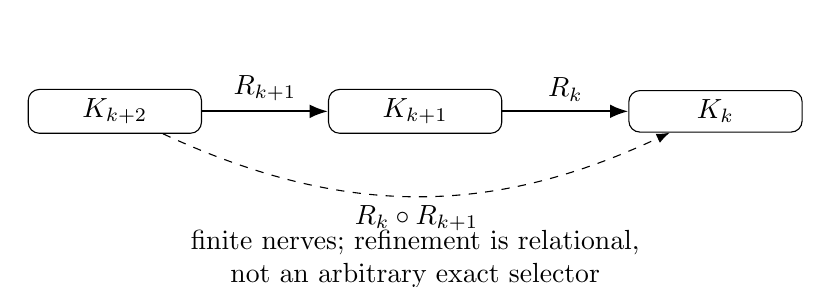
\begin{tikzpicture}[node distance=1.6cm,>=Latex]
  \node (k2) [draw,rounded corners,minimum width=2.2cm] {$K_{k+2}$};
  \node (k1) [draw,rounded corners,minimum width=2.2cm,right=of k2] {$K_{k+1}$};
  \node (k0) [draw,rounded corners,minimum width=2.2cm,right=of k1] {$K_k$};
  \draw[->,thick] (k2) -- node[above] {$R_{k+1}$} (k1);
  \draw[->,thick] (k1) -- node[above] {$R_k$} (k0);
  \draw[->,dashed,bend right=25] (k2) to node[below] {$R_k\circ R_{k+1}$} (k0);
  \node[below=1.1cm of k1,align=center] {finite nerves; refinement is relational,\\not an arbitrary exact selector};
\end{tikzpicture}
\end{center}

\subsection{Presented points}

A point of a represented space can be observed at scale $k$ by a nonempty simplex $O_x(k)$ of $K_k$.  It contains every basic cell consistent with the current finite information.  Coherence means that
\[
  O_x(k)\subseteq R_k(O_x(k+1))
\]
up to the appropriate bitset relation, with a converse ``no observation is lost'' clause when the presentation needs it.  The observation is a cloud, not a single cell.

For a fixed point name, $k\mapsto O_x(k)$ is a fixed primitive-recursive evaluator.  A variable point can be passed by a finite observation table at the current demand horizon.  If an application can prove that $O_x(k)$ eventually becomes a singleton, it may recover an exact cell.  The general theory does not assume this.

\subsection{Presented maps}

\begin{definition}[Tower map]
A tower map $F:\mathcal X\to\mathcal Y$ consists of:
\begin{enumerate}
  \item a primitive-recursive precision demand $\mu_F(k)$;
  \item carriers
  \[
    F_k:K^{\mathcal X}_{\mu_F(k)}\multimap K^{\mathcal Y}_k;
  \]
  \item a finite coherence certificate saying that refining the source and then applying $F_k$, or applying a finer $F_{k+1}$ and then refining the target, gives two selections carried by a common carrier.
\end{enumerate}
\end{definition}

The last clause is naturality up to contiguity.  Strict equality of chosen vertex maps is neither needed nor desirable.  At the chain level, contiguity yields a finite homotopy, so the induced homology map is strictly well defined.

\subsection{How classical spaces produce towers}

Suppose a presented space $X$ comes with finite covers
\[
  \mathcal U_k=\{U_{k,0},\ldots,U_{k,N(k)-1}\}
\]
and finite certificates for nonempty intersections.  Let $K_k$ be the nerve.  Suppose every fine open $U_{k+1,j}$ has a nonempty finite list of certified coarse containers $U_{k,i}$.  Let $R_k(j)$ be that list.  If fine opens $U_{k+1,j}$ for $j\in\sigma$ meet at a point $x$, every chosen coarse container also contains $x$.  Hence their union is a simplex of the coarse nerve.  Thus $R_k$ is a strong carrier.

Now let $f:X\to Y$ have an explicit uniform continuity modulus.  Choose a source scale $\mu(k)$ fine enough that $f(U_{\mu(k),i})$ is contained in at least one target basic open of scale $k$.  Let $F_k(i)$ be the finite list of all certified containers.  If source cells in $\sigma$ meet at $x$, all target containers attached to them contain $f(x)$, so their union is a target simplex.  Again $F_k$ is a strong carrier.

This proof is entirely local and finite.  Abstract compactness is used only in the external theorem that produces the finite covers and a computable modulus.  Inside \ipra, those data are explicit symbols or certificate fields.

\subsection{Pointfree interpretation}

The tower may be used without a pre-existing set of points.  Its vertices are basic observations, its simplices are positive finite intersections, and its refinement carriers are cover relations.  This is close in spirit to formal topology, where basic opens, covers, and positivity are primary and arbitrary point sets are not assumed \cite{Sambin}.  It is also compatible with represented-space practice, where topological properties are expressed through the computability of operations on names and open information \cite{Pauly2016}.

The present construction is deliberately more finitary: at each requested scale, only a finite complex and finite carrier are manipulated.  This is what makes quantifier-free induction and bounded verification available.


\section{The carrier calculus and choice-independent invariants}
\label{sec:carriers}

\subsection{Composition}

\begin{theorem}[Carrier composition]
\label{thm:carrier-composition}
If $C:K\multimap L$ and $D:L\multimap M$ are strong carriers, then $D\circ C:K\multimap M$ is a strong carrier.  Composition is associative, and singleton identity clouds are identities.
\end{theorem}

\begin{proof}
For every source vertex $v$, $C(v)$ is nonempty and every $D(w)$ with $w\in C(v)$ is nonempty.  Therefore their finite union $(D\circ C)(v)$ is nonempty.

Let $\sigma$ be a simplex of $K$.  By the carrier property for $C$,
\[
  \tau=C(\sigma)=\bigcup_{v\in\sigma}C(v)
\]
is a simplex of $L$.  Apply the carrier property for $D$ to $\tau$:
\[
  D(\tau)=\bigcup_{w\in\tau}D(w)
\]
is a simplex of $M$.  Reassociating finite unions gives
\[
  D(\tau)
  =\bigcup_{v\in\sigma}\bigcup_{w\in C(v)}D(w)
  =(D\circ C)(\sigma).
\]
Hence the composite is a carrier.  Associativity and identity follow from associativity and identity of finite union.  Every equality can be proved bit-by-bit by bounded induction.
\end{proof}

\subsection{Selections and contiguity}

\begin{definition}[Selection]
A selection of $C:K\multimap L$ is a vertex map $f:V(K)\to V(L)$ with $f(v)\in C(v)$ for all $v$.
\end{definition}

The least member of each nonempty finite cloud gives a canonical primitive-recursive selection.  This selection is used for execution; correctness does not depend on it.

\begin{theorem}[Selection theorem]
\label{thm:selection}
Every selection $f$ of a strong carrier $C:K\multimap L$ is simplicial.  Any two selections $f,g$ are contiguous: for every simplex $\sigma$ of $K$, the vertex set
\[
  f(\sigma)\cup g(\sigma)
\]
is a simplex of $L$.
\end{theorem}

\begin{proof}
For each $v\in\sigma$, $f(v)\in C(v)$.  Hence
\[
  f(\sigma)\subseteq \bigcup_{v\in\sigma}C(v)=C(\sigma).
\]
The right side is a simplex by the carrier condition, and every subset of a simplex is a simplex.  Thus $f$ is simplicial.

The same argument applied simultaneously to $f$ and $g$ gives
\[
  f(\sigma)\cup g(\sigma)\subseteq C(\sigma),
\]
so the union is a simplex.  This is exactly contiguity.
\end{proof}

\subsection{Chains over $\Ftwo$}

For an ordered finite complex $K$, let $C_q(K;\Ftwo)$ be the finite-dimensional vector space with basis the $q$-simplices.  The boundary is
\[
  \partial[v_0,\ldots,v_q]
  =\sum_{i=0}^{q}[v_0,\ldots,\widehat{v_i},\ldots,v_q]
\]
with coefficients modulo $2$.  Each $(q-2)$-face appears exactly twice in $\partial^2$, so $\partial^2=0$.

A simplicial vertex map $f$ sends a simplex to the sorted set of image vertices; if two source vertices have the same image, the normalized term is zero.  Extending linearly gives a chain map $f_\#$.

All operations are bounded parity folds over finite simplex tables.  No quotient type is needed inside arithmetic: a chain is simply a bitset indexed by the enumerated simplices.

\subsection{The prism operator}

Let $f,g:K\to L$ be contiguous.  For a basis simplex $\sigma=[v_0,\ldots,v_q]$, define over $\Ftwo$
\[
  P_q(\sigma)=
  \sum_{i=0}^{q}
  [f(v_0),\ldots,f(v_i),g(v_i),\ldots,g(v_q)],
\]
where a term with a repeated vertex is normalized to zero.  Contiguity ensures that every nondegenerate term is a simplex of $L$.

\begin{theorem}[Finite prism identity]
\label{thm:prism}
For contiguous simplicial maps $f,g:K\to L$,
\[
  \partial P+P\partial=f_\#+g_\#
\]
as maps of mod-$2$ chain complexes.
\end{theorem}

\begin{proof}
Fix $\sigma=[v_0,\ldots,v_q]$ and expand $\partial P_q(\sigma)$.  A term of $P_q(\sigma)$ has an $f$-block ending at $v_i$ and a $g$-block beginning at the same $v_i$.  Deleting a vertex strictly inside the $f$-block or strictly inside the $g$-block produces exactly the corresponding term of $P_{q-1}(\partial\sigma)$.  These terms therefore occur once in $\partial P$ and once in $P\partial$ and cancel modulo $2$.

At the seam, deleting $g(v_i)$ from the $i$-th prism term produces the same normalized simplex as deleting $f(v_{i+1})$ from the $(i+1)$-st prism term.  These adjacent seam terms also cancel in pairs.  The two unpaired end terms are obtained by deleting $f(v_0)$ from the first prism and deleting $g(v_q)$ from the last prism.  They are precisely $g_\#(\sigma)$ and $f_\#(\sigma)$.  Thus
\[
  (\partial P+P\partial)(\sigma)=f_\#(\sigma)+g_\#(\sigma).
\]

If a tuple has repeated vertices, normalization maps it to zero.  The cancellation pairing respects this normalization: paired words have the same multiset of vertices, so either both normalize to the same simplex or both vanish.  Therefore the identity survives degeneracies.  Linearity proves it for every chain.

For formalization, the preceding prose becomes a bounded index pairing.  Each emitted term is tagged by $(i,j)$, where $i$ is the prism seam and $j$ is the deleted position.  A primitive-recursive involution pairs every tag except the two endpoints; a parity fold proves cancellation by quantifier-free induction.
\end{proof}

\begin{corollary}[Choice-independent homology map]
\label{cor:choice-independent}
Any two selections of a strong carrier induce the same map
\[
  H_q(K;\Ftwo)\longrightarrow H_q(L;\Ftwo)
\]
for every $q$.
\end{corollary}

\begin{proof}
Let $z$ be a cycle.  By \cref{thm:prism},
\[
  f_\#z+g_\#z=\partial Pz+P\partial z=\partial Pz.
\]
Thus $f_\#z$ and $g_\#z$ differ by a boundary and represent the same homology class.
\end{proof}

\subsection{Functorial tower homology}

Every refinement carrier $R_k:K_{k+1}\multimap K_k$ now induces a canonical homology map $r_k$, because the chosen selection is irrelevant by \cref{cor:choice-independent}.  Composition of carriers induces composition of homology maps: selecting from a composite and composing selections are both selections of a common composite carrier, hence contiguous.

\begin{theorem}[Tower homology]
\label{thm:tower-homology}
A certified observation tower determines, for every $q$, an inverse system of finite-dimensional $\Ftwo$-vector spaces
\[
  \cdots\longrightarrow H_q(K_{k+1};\Ftwo)
  \xrightarrow{r_k}
  H_q(K_k;\Ftwo)
  \longrightarrow\cdots.
\]
A coherent tower map determines a morphism of inverse systems, independent of all finite selections.  Composition of tower maps is functorial.
\end{theorem}

\begin{proof}
Choose least selections for execution.  The refinement maps are well defined on homology by \cref{cor:choice-independent}.  The coherence certificate for a tower map says that the two finite vertex maps around each naturality square are carried by a common carrier.  They are therefore contiguous and induce equal homology maps.  This is exactly commutativity of the square on homology.  Carrier composition represents map composition, and \cref{thm:carrier-composition,cor:choice-independent} prove associativity and independence of all selection choices.
\end{proof}

\subsection{Integer coefficients}

Integer chains require signs.  One can use the signed prism
\[
  P_q(\sigma)=\sum_{i=0}^{q}(-1)^i
  [f(v_0),\ldots,f(v_i),g(v_i),\ldots,g(v_q)]
\]
and the identity $\partial P+P\partial=g_\#-f_\#$.  Signed integers are coded by pairs of naturals or a parity-magnitude code.  Homology groups can be computed by Smith normal form.

For \ipra, the easiest robust interface is a \emph{checked Smith certificate}: matrices $U,D,V$ with $UAV=D$, determinants $\pm1$, diagonal $D$, and the divisibility chain.  A bounded verifier checks the certificate.  A separate bounded Euclidean algorithm may produce it when desired.  The mod-$2$ theory is the minimal core because Gaussian elimination and parity cancellation are especially transparent.

\subsection{Acyclic carriers as an extension}

Strong carriers may be generalized.  Assign to each source simplex $\sigma$ a target subcomplex $A(\sigma)$ with face monotonicity and a supplied finite contraction or acyclicity certificate.  The usual acyclic-carrier induction constructs a chain map and a chain homotopy \cite{Munkres}.  In \ipra, ``acyclic'' must not be an unexamined semantic adjective: the certificate must provide bounded filling operators in the required dimensions.  The strong carrier is the special case where $A(\sigma)$ is one simplex and filling is canonical.


\section{Finite topology inside \ipra}
\label{sec:finite-topology}

Finite topological spaces are a useful exact test: no limiting representation is required, yet nontrivial homotopy and homology already occur.  McCord showed that finite spaces and finite simplicial complexes capture the same weak homotopy types in a precise sense \cite{McCord1966}.  For \ipra, the key point is even more elementary: a finite topology has a compact preorder presentation.

\subsection{From a finite topology to a preorder}

Let $X=\{0,\ldots,n-1\}$ and let $\tau$ be a finite topology, coded as a finite list of bitsets.  For $x\in X$, define its minimal open neighborhood
\[
  U_x=\bigcap\{U\in\tau:x\in U\}.
\]
The intersection is finite, hence open.  Define
\[
  x\preceq y
  \quad\Longleftrightarrow\quad
  y\in U_x,
\]
equivalently: every open set containing $x$ also contains $y$.

\begin{theorem}[Finite topology/preorder equivalence]
\label{thm:finite-preorder}
The relation $\preceq$ is a preorder.  The open sets of $\tau$ are exactly the upward-closed subsets for $\preceq$.  Conversely, the upward-closed subsets of any finite preorder form a topology.  These constructions are mutually inverse.  The topology is $T_0$ exactly when the preorder is antisymmetric.
\end{theorem}

\begin{proof}
Reflexivity holds because $x\in U_x$.  If $x\preceq y$ and $y\preceq z$, every open containing $x$ contains $y$, and then contains $z$; hence $x\preceq z$.

Every open $U$ is upward closed: if $x\in U$ and $x\preceq y$, the definition of $\preceq$ gives $y\in U$.  Conversely let $A$ be upward closed.  For each $x\in A$, $U_x\subseteq A$, because $y\in U_x$ means $x\preceq y$.  Since $x\in U_x$, we have
\[
  A=\bigcup_{x\in A}U_x,
\]
so $A$ is open.

For a preorder, arbitrary unions and finite intersections of upward-closed sets are upward closed, so they form a topology.  Its minimal neighborhood of $x$ is $\{y:x\preceq y\}$, recovering the relation.

Finally, $x$ and $y$ have the same open neighborhoods exactly when $x\preceq y$ and $y\preceq x$.  The $T_0$ axiom says this forces $x=y$, which is antisymmetry.
\end{proof}

Every assertion in the proof is a bounded formula over $x,y,z<n$ and bit membership.  Therefore \cref{thm:booleanization} and quantifier-free induction suffice for a direct object proof.

\subsection{Continuous maps are monotone maps}

\begin{theorem}[Finite continuity]
\label{thm:finite-continuity}
For finite spaces presented by their specialization preorders, a function $f:X\to Y$ is continuous if and only if it is monotone:
\[
  x\preceq_X x'\ \Longrightarrow\ f(x)\preceq_Y f(x').
\]
\end{theorem}

\begin{proof}
Assume $f$ is continuous and $x\preceq_X x'$.  Let $V$ be any open neighborhood of $f(x)$.  Then $f^{-1}(V)$ is open and contains $x$, so it contains $x'$.  Thus $f(x')\in V$.  Since this holds for every such $V$, $f(x)\preceq_Y f(x')$.

Conversely assume $f$ is monotone and $V\subseteq Y$ is upward open.  If $x\in f^{-1}(V)$ and $x\preceq_X x'$, monotonicity gives $f(x)\preceq_Y f(x')$.  Upward closure of $V$ yields $f(x')\in V$, so $f^{-1}(V)$ is upward open.
\end{proof}

The preorder encoding is exponentially smaller than listing all open sets in the worst case and makes continuity a bounded pairwise condition.  It is therefore the preferred exact finite representation.

\subsection{Basic constructions}

All of the following are primitive-recursive on finite codes.

\paragraph{Products.}
The product preorder on $X\times Y$ is coordinatewise:
$(x,y)\preceq(x',y')$ iff $x\preceq x'$ and $y\preceq y'$.  The standard product topology on finite spaces is recovered.

\paragraph{Subspaces.}
For a bitset $A\subseteq X$, restrict the preorder to selected vertices.  A coded reindexing produces a finite preorder on $\{0,\ldots,|A|-1\}$.

\paragraph{Quotients.}
Given a finite equivalence relation $E$ compatible with the preorder, choose the least representative of each class and define the quotient relation by bounded existential search.  A verifier checks well-definedness and the universal property for supplied maps.

\paragraph{Connected components.}
The undirected comparability graph has an edge between $x$ and $y$ when $x\preceq y$ or $y\preceq x$.  Its graph components are the topological connected components of a finite space.  Breadth-first search with a visited-bitset invariant computes them.

\paragraph{Order complex.}
For a finite $T_0$ space, the order complex has a simplex for every finite chain $x_0<\cdots<x_q$.  Its construction is bounded.  It supplies the bridge from finite spaces to simplicial homology used in McCord's theory \cite{McCord1966}.

\subsection{What finite topology does and does not solve}

Finite spaces provide exact models, regression tests, and finite approximants.  They do not imply that every infinite topological theorem reduces to one finite space.  The missing information is carried by the observation tower: how finite covers refine, how maps act at every requested scale, and what quantitative condition connects the tower to the intended space.


\section{A topology library built from finite certificates}
\label{sec:library}

This section lists the principal topological notions and gives an \ipra-compatible formulation.  The goal is not to force all topology into one definition, but to expose exactly which finite observations and positive certificates each theorem uses.

\subsection{Open information and continuity}

At scale $k$, a basic open is a vertex of $K_k$.  A finite union is a bitset.  Membership of a presented point is positive when its observation simplex meets the bitset in a certified way.  Arbitrary subsets of points are not internal objects.

A continuous map is represented by a modulus and carriers as in \cref{sec:towers}.  This formulation has three advantages:
\begin{enumerate}
  \item it is pointfree at the finite level;
  \item it permits multiple valid target cells at boundaries;
  \item composition is finite relational composition.
\end{enumerate}

For metric presentations, the familiar evaluator/modulus formulation induces the carrier formulation.  Conversely, if the tower is spatially complete and has a shrinking mesh, a coherent carrier map determines the usual continuous action on regular point names.  That converse is a semantic theorem about the chosen presentation, not a generic fact of first-order arithmetic.

\subsection{Compactness}

Abstract compactness says every open cover has a finite subcover.  Quantifying over arbitrary open covers is higher-type and often nonconstructive.  The usable data are instead:

\begin{definition}[Finite compactness contract]
A compactness contract supplies a primitive-recursive net $N(k)$, a finite cover $\mathcal U_k$, and a verifier proving that every represented point is observed in at least one member, with mesh or Lebesgue data sufficient for the intended theorem.
\end{definition}

If an application receives a finite candidate cover by basic opens, coverage reduces to a bounded statement about the net plus a supplied uniform-continuity or inclusion margin.  Bounded search extracts a subcover when the list is redundant.  The contract does not turn an arbitrary infinite enumeration of opens into a finite subcover without a bar, modulus, or stopping bound.

\subsection{Separation and apartness}

A Hausdorff-style effective presentation supplies a separation procedure:
\[
  \operatorname{Apart}(x,y,s)=1
  \Longrightarrow
  \text{disjoint basic neighborhoods of scale }s.
\]
For regular fast metric names, a witnessed lower distance bound provides this procedure.  Negated name equality alone does not.

At the tower level, two observation clouds are apart at scale $k$ when no simplex contains a vertex from each cloud, or when an explicit disjointness certificate is supplied.  Separation propagates under refinement by a bounded proof.

\subsection{Connectedness and paths}

There are several constructive strengths.

\begin{definition}[Finite chain connection]
Two vertices of $K_k$ are chain connected when they lie in the same component of the $1$-skeleton.  A certificate is a finite vertex path whose consecutive pairs are edges.
\end{definition}

A presented space is \emph{uniformly chain connected} when a fixed primitive-recursive procedure produces such paths between observation clouds at every requested scale.  This positive statement is stronger and more computational than merely denying a separation into two opens.

A represented path is a tower map from an interval tower.  Polygonal paths with rational vertices are especially convenient: evaluation, subdivision, and clearance tests are primitive recursive.  Homotopies are tower maps from a product with an interval tower.

\subsection{Products}

Given covers $\mathcal U_k$ and $\mathcal V_k$, use the product cover $U_i\times V_j$.  A finite family of product cells has nonempty intersection exactly when both coordinate families do, provided the factor intersection certificates are available.  Thus the product nerve is a finite combinatorial construction on pairs.  Refinement and map carriers are componentwise.

The construction proves that products of certified towers are certified towers.  For metric spaces, the max metric gives a simple mesh bound.  All dimension bounds, bitset encodings, and demand transformations are explicit.

\subsection{Subspaces and closed conditions}

A subspace cannot in general be formed merely from a negative predicate.  The tower needs a positive answer to ``which cells meet the subspace?''  Suitable inputs include:
\begin{itemize}
  \item a finite decidable subset of a finite space;
  \item an zero set with isolating boxes and sign/degree certificates;
  \item a compact set with a distance-name and positive intersection witnesses;
  \item a supplied finite subcomplex.
\end{itemize}
Cells with certified intersection become vertices; inherited intersection certificates define the subcomplex.  Ambiguous cells remain as clouds rather than being discarded.

\subsection{Quotients}

For finite spaces and finite complexes, quotients by a decidable equivalence relation are bounded constructions.  For represented spaces, a quotient presentation requires more:
\begin{enumerate}
  \item a fixed evaluator for the equivalence relation or orbit action;
  \item finite saturation of observation clouds;
  \item compatibility of refinement;
  \item separation data if a Hausdorff quotient is claimed.
\end{enumerate}
Without these fields, a quotient may destroy effective separation or make equality undecidable.  The framework therefore treats quotient quality as a certificate, not as an automatic theorem.

\subsection{Homology and cohomology}

At each scale, mod-$2$ homology is computed from finite boundary matrices.  Gaussian elimination is a bounded loop.  Its invariant records:
\begin{itemize}
  \item the processed pivot columns;
  \item preservation of row space under elementary operations;
  \item pivot distinctness;
  \item rank accounting.
\end{itemize}
The Betti formula is
\[
  \beta_q(K)=n_q-\operatorname{rank}\partial_q-
  \operatorname{rank}\partial_{q+1}.
\]

Cohomology uses transposed boundary matrices.  Cup products are finite formulas on simplex tables; associativity and the Leibniz rule can be proved by bounded index manipulations.  Integral torsion is added by checked Smith certificates as described after \cref{thm:prism}.

The tower does not force Betti numbers to stabilize.  Stabilization, pro-isomorphism, or identification with singular/Cech homology is a semantic theorem requiring hypotheses on the cover system.  McCord's finite-space results and classical nerve theorems indicate the relevant bridges \cite{McCord1966}, but each effective use must supply finite good-cover or acyclicity certificates.

\subsection{Fundamental groups}

For a finite complex, an edge loop is a finite list of vertices.  Elementary edge homotopies insert or delete backtracks and triangle moves.  A bounded sequence of such moves is a positive null-homotopy certificate.  Van Kampen presentations can be produced from a finite spanning tree and $2$-simplex relations.

What is not available uniformly is a decision procedure for the word problem in arbitrary finitely presented groups.  The \ipra\ interface is therefore asymmetric:
\begin{itemize}
  \item a supplied bounded homotopy is verifiable;
  \item bounded search can find one below a stated bound;
  \item absence of a bounded certificate is not a proof of non-null-homotopy;
  \item special classes with a proven normal-form algorithm may add a decision contract.
\end{itemize}

\subsection{Manifolds and atlases}

A compact effective $d$-manifold can be presented by a finite atlas at each scale:
\[
  (U_i,\phi_i,\psi_i,r_i),
\]
where $\phi_i$ and $\psi_i$ are fixed rational evaluators for a chart and its inverse on guarded domains, $r_i$ is a positive interior margin, and overlap transitions have explicit moduli.  Finite cover certificates prove that the shrunken chart domains cover the space.  Carriers handle points lying in several charts.

Local topological proofs reduce to rational boxes.  Differential topology adds rational derivative names, determinant gaps for inverse-function steps, and transversality margins.  Smooth partitions of unity require explicit bump-function approximants and denominator lower bounds.  None of these should be hidden inside the word ``smooth.''

For noncompact manifolds, add a primitive-recursive exhaustion by compact charted pieces.  A theorem at precision $k$ advertises the exhaustion stage it needs.  This is the same finite-demand discipline used throughout.

\subsection{Fixed-point theorems}

A Sperner labeling on a finite triangulation is a bounded object.  The parity proof yields an approximate fixed-point simplex.  Given a uniformly continuous map on a compact presented simplex, a mesh choice turns this into
\[
  \|f(x)-x\|<2^{-k}
\]
for an explicitly produced rational point $x$.

An exact fixed point is a different claim.  To construct a coherent name, one needs nested compatible approximate witnesses.  This can be obtained from an isolation/uniqueness modulus, from a relational viability dynamic program, or from an explicit compact choice principle available for the particular presentation.  Unrelated approximate fixed points at each scale do not automatically form one point.

\subsection{Dimension and local degree}

Dimension obstructions are particularly suitable for finite topology.  The repository's staggered-grid theorem is already a quantitative finite alternative.  Invariance of domain can be approached similarly: triangulate a rational box, represent a map by a sufficiently fine carrier, compute a local mod-$2$ degree on a boundary complex, and use an injectivity-separation modulus to prevent cancellation.  The finite degree calculation is within \ipra; producing the required uniform separation data is the substantive application hypothesis.

One must not silently infer unrestricted classical invariance theorems from the finite core.  Reverse-mathematical work shows that some unrestricted Brouwer invariance statements have weak-Koenig-lemma strength over standard base theories \cite{Kihara2020}.  The present goal is the maximal explicit, effectively presented version: fixed evaluators, positive moduli, and finite certificates.


\section{Topology case studies}
\label{sec:cases}

\subsection{The Sierpinski space}

Let $X=\{0,1\}$ with preorder $0\preceq1$ and no converse relation.  The upward opens are
\[
  \varnothing,\quad\{1\},\quad\{0,1\}.
\]
The exact Python kernel reconstructs these opens from the relation.  Exhaustive enumeration of all maps between three representative two-point preorders confirms the theorem ``monotone iff continuous'' in every case; the human proof is \cref{thm:finite-continuity}.

This example is small but instructive.  Open information is directional: observing $0$ forces compatibility with $1$.  A preorder code expresses this directly, while an open-set list obscures it.  It also illustrates why non-Hausdorff finite spaces remain topologically meaningful.

\subsection{A carrier tower for the circle}

Let $C_n$ be the one-dimensional cycle complex with vertices $0,\ldots,n-1$ and edges $\{j,j+1\bmod n\}$.  Define a binary refinement carrier
\[
  R:C_{2n}\multimap C_n
\]
by
\[
  R(2i)=\{i\},
  \qquad
  R(2i+1)=\{i,i+1\bmod n\}.
\]
For every fine edge, the union of its endpoint clouds is one coarse edge, so $R$ is a strong carrier.

There are two obvious selections: choose the smaller or the larger endpoint of each ambiguous cloud.  They differ exactly at subdivision vertices.  By \cref{thm:selection}, both are simplicial and contiguous.  The prism theorem proves they induce the same map on $H_1$.  The exact kernel verifies
\[
  \beta(C_4)=\beta(C_8)=\beta(C_{16})=(1,1)
\]
and checks the prism matrix identity for the two selections.

This is the model for a boundary point in a cover: the point belongs to two adjacent cells, and no exact convention should affect the topological invariant.

\subsection{Jordan separation}

The constructive Jordan theorem is naturally expressed with positive clearance.  Let $\gamma$ be a circle embedding with:
\begin{itemize}
  \item a fixed rational approximation evaluator;
  \item a forward continuity modulus;
  \item an inverse separation modulus ensuring that separated parameters have separated images.
\end{itemize}
For a rational query point $p$ with a positive lower distance bound from the curve, a sufficiently fine polygonal approximation has stable crossing parity.  Triangle replacement proves independence from further refinement.  A finite grid or honeycomb flood computes a route within the equal-parity region; failure would extract a separating cycle whose parity change contradicts equality of the endpoint bits.  This is the constructive strategy of Berg--Julian--Mines--Richman in finite arithmetic form \cite{Berg1975}, consistent with the discrete bounded-arithmetic analyses of Nguyen and Cook \cite{NguyenCook} and later constructive treatments \cite{Bridges2025}.

The carrier framework improves the interface in four ways.

\begin{enumerate}
  \item A curve sample lying on a grid boundary belongs to all adjacent safe cells.  Keep that cloud rather than imposing a global tie-break.
  \item Polygon refinements are carriers between finite cycle complexes.  Crossing parity invariance is a finite chain statement.
  \item Safe-region routes are finite edge chains in a complement complex; alternative routing choices are related by finite $2$-cell fillings when available.
  \item The inside/outside bit is defined on the apartness complement.  No decision at zero clearance is asserted.
\end{enumerate}

A complete object proof still needs the theorem-specific crossing and flood-fill invariants.  The tower/carrier library removes repeated map-choice, refinement, and homology bookkeeping; it does not replace the Jordan parity argument itself.

\subsection{Invariance of dimension}

For a presented map $f:[0,1]^d\to\R^m$, choose a rational grid fine enough that the oscillation on each Kuhn simplex is below a requested threshold.  Encode its vertex values as rational integer tuples after clearing denominators.  The repository's finite theorem gives the positive alternative:
\begin{quote}
if $d>m$, then either opposite source faces have images closer than the claimed separation, or one Kuhn simplex has image oscillation at least the local bound.
\end{quote}
Both conclusions are finite witnesses.  Applied to a presented homeomorphism and its inverse with explicit moduli, they force equality of dimensions.

In the tower language, Kuhn triangulations are levels, subdivision is a refinement carrier, and the map evaluator induces a target-grid carrier.  Staggered grid labels are Boolean functions on vertices.  The cubical Sperner parity theorem becomes a reusable finite contract.  Boundary ambiguity is harmless because adjacent target cells form a carrier simplex.

The restriction to explicitly presented maps is essential.  The statement is a schema for fixed evaluators and moduli, not a first-order universal quantification over all real functions.  This matches the logical boundary highlighted by the existing packet and by reverse-mathematical results on unrestricted invariance principles \cite{Kihara2020}.

\subsection{Nerve computations from good covers}

Suppose a compact presented space has a finite cover $\mathcal U$ such that every nonempty finite intersection comes with a contraction certificate.  The nerve $N(\mathcal U)$ is finite.  An effective nerve theorem can be organized by two acyclic carriers:
\begin{enumerate}
  \item a carrier from a sufficiently fine spatial triangulation to the nerve, assigning all cover elements containing a cell;
  \item a carrier back, using supplied contraction/filling operators for cover intersections.
\end{enumerate}
The carrier composites are chain homotopic to identities.  Therefore the finite nerve and the spatial complex have isomorphic homology.  If the intersections are literally represented by one simplex at the finite level, strong carriers suffice; otherwise use the certified acyclic extension.

The phrase ``good cover'' must therefore expand to finite data: an intersection table, positivity witnesses, and bounded contractions or filling matrices.  With those fields, the proof is finite and \ipra-compatible.

\subsection{Surfaces and Euler characteristic}

A triangulated compact surface is a finite complex with local-link certificates.  The Euler characteristic
\[
  \chi=V-E+F
\]
is exact integer arithmetic.  Edge-incidence checks verify that each edge has two incident faces in the closed case, and vertex links verify the local manifold condition.  Mod-$2$ Betti numbers provide
\[
  \chi=\beta_0-\beta_1+\beta_2.
\]
The equality follows from rank cancellation in the finite chain complex and is formalizable by bounded matrix arithmetic.

Classification of surfaces requires more: a finite sequence of certified elementary moves reducing a triangulation to a normal form, or an algorithm with a well-founded finite measure and invariant.  The framework can verify such traces and prove their invariants.  It does not treat the classification theorem as a one-line consequence of coding.


\section{Resolution of recurring difficulties beyond topology}
\label{sec:cross-domain}

The carrier idea is topological in origin but addresses a general problem: finite evidence may determine a compatible family rather than a unique output.  This section records how the framework applies across the repository.

\subsection{Root and eigenvalue collisions}

At precision $k$, let vertices be rational boxes or spectral intervals.  A simplex is a jointly compatible cluster.  Refinement relates fine isolating boxes to every coarse box containing them.  Polynomial evaluation or a matrix algorithm returns a carrier of possible clusters.

Symmetric observables---root multisets, elementary symmetric functions, spectral projectors separated by a gap---are invariant under selections.  An individual ordered root or eigenvector is produced only when an isolation or apartness certificate collapses the cloud.  This avoids exact choice at collisions and matches the existing root-cluster and stable-observable recommendations.

\subsection{Local analytic branches}

A local implicit-function proof typically has several overlapping rational charts.  Let vertices be certified chart domains; a simplex means a common subdomain is nonempty.  Transition maps form carriers because a point on a chart boundary may admit several valid target charts.  Carrier composition proves that finite analytic continuation does not depend on tie-breaking, while a monodromy invariant can be computed on the resulting nerve.

The producer still needs a simple-root or invertible-Jacobian gap.  At a singular point, a chart cloud may fail to contract to one branch.  The framework represents this honestly rather than asserting a hidden selector.

\subsection{Integration and measure}

Use finite partitions with rational interval enclosures for function values and cell masses.  Refinement carriers relate subcells to containing cells.  Lower and upper sums are finite rational folds.  A modulus or variation bound controls the gap.  Measures are not quantified as arbitrary higher-type functionals; a fixed mass evaluator and additivity certificates are supplied.

Discontinuous tests, such as a cumulative distribution function exactly at an atom, require an anti-concentration margin or one-sided interval output.  A relational interval is the measure-theoretic analogue of a carrier cloud.

\subsection{Diophantine finiteness}

For a bounded region, candidate points form a finite complex with discrete vertices.  A verifier can check equations and distinctness.  A height certificate turns qualitative finiteness into complete bounded enumeration.  Carrier methods help with local charts or descent representatives, but they do not produce the height bound.

Thus the correct contract remains:
\[
  \text{height/cover producer}
  \quad+\quad
  \text{finite enumeration verifier}.
\]
The framework clarifies exactly which part is missing in general Siegel- or Faltings-type applications.

\subsection{Prime-distribution and analytic constants}

A finite verifier can check zero-free rectangles, explicit coefficient inequalities, or an exceptional-zero certificate.  It cannot derive ineffective constants from a qualitative classical theorem.  The theorem should be parameterized by an analytic-input certificate whose fields are consumed by bounded computations.  Precision demands are propagated backward through the contract graph.

\subsection{Metastability and convergence}

A metastable window theorem returns, for every control function and precision, a finite stable interval.  It does not automatically return a Cauchy modulus.  Observation towers record windows and their refinement compatibility.  A coherent limit name requires additional uniqueness or compactness data.  This prevents an invalid conversion from ``there are arbitrarily stable windows'' to ``there is a computable final stage.''

\subsection{A unified difficulty matrix}

\begin{longtable}{@{}p{0.20\textwidth}p{0.31\textwidth}p{0.38\textwidth}@{}}
\toprule
Difficulty & Invalid shortcut & Framework response \\
\midrule
\endfirsthead
\toprule
Difficulty & Invalid shortcut & Framework response \\
\midrule
\endhead
Arbitrary functions or spaces & Quantify over evaluator codes and assume a universal PR evaluator & Fixed-symbol schemas, finite tables, or clocked traces \\
All-precision induction & Induct on a Cauchy statement containing unbounded quantifiers & Fix precision, compute a finite demand horizon, Booleanize the finite table \\
Exact boundary choice & Choose one containing cell, root, chart, or axis globally & Return a carrier cloud; select only for execution; prove invariant independence by contiguity/prism \\
Abstract compactness & Invoke a finite subcover without a bound & Supply finite nets/covers, a Lebesgue or mesh modulus, and a bounded coverage verifier \\
Semantic Lean proof & Apply native transport to an ambient theorem & Build an actual $\Prf\ \PRAAx$ term, then apply \code{pra\_iff\_native} \\
Finiteness without cutoff & Enumerate until nothing new appears & Separate bound producer from finite verifier; accept explicit height/exhaustion certificate \\
Ineffective constants & Treat existence as a numerical input & Parameterize by a checked analytic certificate with correct quantifier order \\
Negated equality & Infer a numerical gap from $x\neq y$ & Require apartness, strict margins, or disjoint basic neighborhoods \\
Map composition at boundaries & Compose independently selected approximants & Compose carriers relationally; naturality holds up to contiguity \\
Homology of approximants & Assume Betti numbers eventually stabilize & Work with the inverse system; prove stabilization or a nerve equivalence as a separate certificate \\
\bottomrule
\end{longtable}

The central pattern is ``do not destroy finite ambiguity prematurely.''  A cloud is often easier to compose, more constructive, and more invariant than a selected representative.


\section{Lean formalization plan}
\label{sec:lean}

\subsection{Target repository interfaces}

The current ProveIt API needed by this work is small:
\begin{itemize}
  \item \code{PR k}: fixed primitive-recursive function syntax;
  \item \code{PTm n}: arithmetic terms;
  \item \code{Fm PTm n}: formulas;
  \item \code{PRAAx}: defining equations, successor axioms, and quantifier-free induction;
  \item \code{Prf}: intuitionistic derivations;
  \item \code{PRA.proj}, \code{PRA.comp}, \code{PRA.precZero}, \code{PRA.precSucc}: defining-equation lemmas;
  \item \code{PRA.qfInd}: object quantifier-free induction;
  \item \code{pra\_iff\_native}: the final native transport.
\end{itemize}

The supplied file \code{lean/IPRAObjectLanguageBlueprint.lean} imports these actual modules and states the intended endpoints.  It deliberately does not replace them by a surrogate proof relation.

\subsection{Phase 1: primitive-recursive data structures}

Implement explicit \code{PR} syntax trees for:
\begin{enumerate}
  \item pair, left, right, list length, bounded list access;
  \item bit membership, bounded union/intersection, popcount;
  \item bounded all/any/search and least witness;
  \item signed integers and mod-$2$ arithmetic;
  \item finite vectors and matrices;
  \item lexicographic enumeration of bitsets and simplices.
\end{enumerate}

For each symbol, prove its defining equations using the existing composition and primitive-recursion lemmas.  Malformed codes return defaults.  Domain predicates are separate Boolean terms.

\subsection{Phase 2: bounded Booleanization}

Define a metalevel inductive syntax of bounded formulas.  Its compiler returns:
\begin{lstlisting}[language={},caption={Required Booleanization interface}]
structure Booleanized (n : Nat) where
  formula    : Fm PTm n
  test       : PR n
  equivalent : [] |- [PRAAx] (formula <-> accepts test)
\end{lstlisting}
The displayed notation is schematic; the actual file uses \code{Fm.iff} and equality with the numeral one.  Prove the compiler correct by syntax recursion.  Bounded quantifier nodes emit finite folds and close them with \code{PRA.qfInd}.

This phase is the most reusable missing component in the repository.  Once it exists, preorder, simplex, carrier, path, and matrix invariants become equalities of Boolean terms.

\subsection{Phase 3: finite complexes and carriers}

Represent a complex by a vertex bound and a simplex-test symbol.  Its contract proves empty-simplex and downward-closure laws.  Represent a carrier by a cloud symbol.  Prove:
\begin{enumerate}
  \item cloud nonemptiness and bounds;
  \item the strong carrier condition;
  \item correctness of least selection;
  \item selection simpliciality;
  \item contiguity of any two bounded selections;
  \item validity and associativity of relational composition.
\end{enumerate}

All formulas are bounded by the vertex counts.  The human proofs in \cref{thm:carrier-composition,thm:selection} translate directly to bitset inclusions and downward closure.

\subsection{Phase 4: finite preorders}

Define a Boolean relation $\leq_X$ and bounded formulas for reflexivity and transitivity.  An open bitset is upward closed.  Define inverse image by a bounded fold.  Formalize \cref{thm:finite-preorder,thm:finite-continuity}.

One convenient route avoids enumerating all $2^n$ opens in the continuity theorem: prove monotonicity implies preservation of every upward bitset by taking an arbitrary numerical bitset variable.  Conversely use the principal upward set $U_{f(x)}=\{y:f(x)\leq y\}$, whose characteristic function is a fixed Boolean term.

\subsection{Phase 5: chain complexes and the prism}

Enumerate $q$-simplices by bounded search over bitsets.  A mod-$2$ chain is a bitset over this enumeration.  Define:
\[
  \partial_q,\quad f_{\#,q},\quad P_q
\]
as bounded parity folds.  Prove:
\begin{enumerate}
  \item $\partial^2=0$ by pairing the two deletion orders;
  \item $f_\#$ commutes with boundary;
  \item the prism identity by the explicit tag involution from \cref{thm:prism}.
\end{enumerate}

The invariant for a parity fold is an equality modulo $2$ between the processed prefix and a specification fold.  It is quantifier-free after Booleanization.

\subsection{Phase 6: homology certificates}

Implement bounded Gaussian elimination over $\Ftwo$.  The state contains the matrix, current row and column, pivot list, and accumulated transformation data.  The invariant states that elementary operations preserve row space and that processed pivots are distinct.  The exit theorem yields rank.

A direct internal quotient construction for homology is unnecessary for numerical Betti results.  For induced-map equality, represent a cycle and two image chains explicitly; the prism provides a boundary witness.  If a reusable finite vector-space quotient API is desired, encode reduced bases and normal forms by elimination certificates.

\subsection{Phase 7: tower schemas}

A generic Lean structure may quantify over host functions $k\mapsto K_k$, but an object-\ipra\ theorem must instantiate fixed symbols or finite prefixes.  Therefore provide two layers:
\begin{enumerate}
  \item semantic structures in \code{TopologySemanticBlueprint.lean};
  \item an object compiler that consumes a finite expression describing a fixed family and emits \code{PR} terms and $\Prf\ \PRAAx$ derivations.
\end{enumerate}

For each requested precision $k$, the theorem computes the finite demand $\mu(k)$ and constructs only the required prefix.  Universal quantification over $k$ is introduced at the end.

\subsection{Phase 8: application modules}

Suggested repository modules are:
\begin{lstlisting}[language={},caption={Proposed module layout}]
ConciseIPRA/Applications/FiniteCoding.lean
ConciseIPRA/Applications/BoundedBoolean.lean
ConciseIPRA/Applications/FinitePreorder.lean
ConciseIPRA/Applications/SimplicialComplex.lean
ConciseIPRA/Applications/Carrier.lean
ConciseIPRA/Applications/ChainsF2.lean
ConciseIPRA/Applications/Prism.lean
ConciseIPRA/Applications/GaussianF2.lean
ConciseIPRA/Applications/ObservationTower.lean
ConciseIPRA/Applications/Topology/JordanKernel.lean
ConciseIPRA/Applications/Topology/DimensionKernel.lean
\end{lstlisting}

The first end-to-end milestone should be small but genuine:
\begin{quote}
construct an object-\ipra\ proof that the two least/maximal selections of the $C_8\multimap C_4$ circle carrier induce homologous images of the fundamental mod-$2$ cycle.
\end{quote}
This exercises bitsets, complexes, selections, chains, boundary, prism, and the native bridge without requiring represented analysis.

\subsection{No false completion claim}

The supplied Lean files are uncompiled and contain explicit \code{sorry} obligations.  The build environment used for this package had no Lean executable.  The Python kernel checks the intended finite definitions but is not a Lean compiler and not an \ipra\ proof checker.  These boundaries are recorded in the theorem ledger.


\section{Executable finite validation}
\label{sec:validation}

\subsection{Reference kernel}

The file \code{code/topology\_kernel.py} is an exact standard-library implementation of:
\begin{itemize}
  \item finite abstract simplicial complexes and downward closure;
  \item strong carriers and relational composition;
  \item least and greatest selections;
  \item mod-$2$ boundary matrices and Gaussian rank;
  \item Betti numbers;
  \item simplicial chain maps;
  \item the mod-$2$ prism operator and matrix identity;
  \item finite preorders, upward opens, monotonicity, and continuity;
  \item finite prefixes of observation towers.
\end{itemize}

All computations use integers and finite sets.  There is no floating-point arithmetic and no random test dependence.

\subsection{Test results}

The delivered run passes 15 unit tests.  They include:
\begin{enumerate}
  \item Betti numbers of an interval, a cycle, and two isolated points;
  \item $\partial^2=0$ on a filled triangle;
  \item mod-$2$ matrix rank;
  \item rejection of an invalid carrier;
  \item chain-map commutation with boundary;
  \item carrier composition and tower composition;
  \item contiguity of least and greatest circle-refinement selections;
  \item the full prism matrix identity;
  \item the Sierpinski topology and the discrete two-point topology;
  \item exhaustive equivalence of monotonicity and continuity for all maps among three representative two-point preorders;
  \item validation of the JSON circle carrier certificate.
\end{enumerate}

The recorded circle certificate has source $C_8$, target $C_4$, Betti vectors $(1,1)$ on both sides, and two distinct selections.  The kernel confirms that the selections are contiguous and that
\[
  \partial P+P\partial=f_\#+g_\#
\]
holds as an equality of finite matrices in every source dimension.

\subsection{What the tests establish}

The tests establish that the supplied reference implementation behaves as described on the covered finite instances.  They are useful for detecting indexing, normalization, parity, and boundary errors.  They do not prove the universal carrier or prism theorems, and they do not check a $\Prf\ \PRAAx$ derivation.  The universal proofs are the human arguments in \cref{sec:carriers}; their formalization path is \cref{sec:lean}.

\subsection{Reproduction}

From the package root:
\begin{lstlisting}[language=bash]
python3 -m unittest -v code/test_topology_kernel.py
python3 code/topology_kernel.py --example
python3 code/topology_kernel.py examples/circle_carrier.json
\end{lstlisting}
The validation directory contains the captured outputs.


\section{Limits, residual obligations, and research directions}
\label{sec:limits}

\subsection{What has been resolved}

At the level of statement design and finite mathematics, the framework resolves the following recurring obstacles.

\begin{enumerate}
  \item \textbf{Boundary ambiguity.}  Replace exact choice by a finite carrier cloud.  Composition remains total, and homology is choice independent.
  \item \textbf{Map composition.}  Relational union composes finite approximations without coordinating arbitrary tie-breaks.
  \item \textbf{Topological invariants.}  The prism identity gives an explicit finite witness that contiguous choices induce the same homology map.
  \item \textbf{Finite topology.}  Preorders give a compact exact coding, and continuity becomes bounded monotonicity.
  \item \textbf{Compactness usage.}  Finite covers, nets, and mesh/Lebesgue certificates replace an unbounded open-cover quantifier.
  \item \textbf{All-precision reasoning.}  Finite demand analysis and Booleanization keep induction quantifier-free.
  \item \textbf{Formal endpoint.}  Every main theorem has a stated $\Prf\ \PRAAx$ target and a dependency order.
\end{enumerate}

\subsection{What remains theorem-specific}

The framework deliberately does not claim completed object proofs for:
\begin{itemize}
  \item cubical Sperner parity and staggered-grid dimension obstruction;
  \item the complete Jordan crossing, flood-fill, and boundary-density argument;
  \item a general effective nerve theorem with produced contraction data;
  \item invariance of domain or general manifold classification;
  \item stabilization of homology for arbitrary observation towers;
  \item production of finite atlases, triangulations, or good covers from weak input presentations.
\end{itemize}
These are mathematical modules to be built on the common kernel.

\subsection{Logical boundaries}

The following stronger principles are not obtained by better coding alone.

\begin{enumerate}
  \item There is no uniform total primitive-recursive evaluator for arbitrary PR program codes.
  \item Negated equality does not uniformly yield a positive apartness scale.
  \item A finite verifier does not produce a missing global bound or modulus.
  \item Independent approximate witnesses at every precision do not necessarily form one coherent point.
  \item Unrestricted classical topological statements may have proof-theoretic strength exceeding the intended finitistic base; effective hypotheses must be stated explicitly \cite{Kihara2020}.
\end{enumerate}

\subsection{Recommended next formal milestones}

The most valuable immediate work is foundational rather than another large theorem outline.

\begin{enumerate}
  \item Complete and compile the bounded Booleanization library in the actual \code{ConciseIPRA} environment.
  \item Formalize strong carriers and the circle refinement example end to end, including the object prism identity.
  \item Add bounded Gaussian elimination and a verified Betti-number contract.
  \item Refactor the Jordan and dimension packets so that their finite complexes and refinement maps use the shared carrier API.
  \item Develop certified acyclic carriers with explicit finite filling operators; this unlocks effective nerve theorems and chain-level local-to-global arguments.
  \item Build a compact metric-space tower interface with rational covers, mesh bounds, positive intersections, and map moduli.
\end{enumerate}

\subsection{Conclusion}

The most robust way to place topology in \ipra\ is not to encode an arbitrary powerset topology as one enormous natural number.  It is to identify the finite observations actually used by a proof, arrange them in certified refinement towers, preserve ambiguity as relational carriers, and compile every finite invariant into bounded Boolean arithmetic.

This yields a coherent division of labor.  Topology supplies covers, nerves, carriers, chain homotopies, and local-to-global structure.  \ipra\ supplies primitive recursion, bounded search, exact arithmetic, and quantifier-free induction.  The representation theorem connecting a tower to a classical or constructive space remains explicit.  The object-language derivation remains explicit.  Under these rules, sophisticated topological arguments can be developed without importing hidden choice, compactness, or higher-type quantification.

\appendix

\section{Explicit coding primitives}
\label{app:coding}

This appendix records one concrete coding route.  Other fixed primitive-recursive codings may be substituted if their laws are proved.

\subsection{Pairs and lists}

Use
\[
  \langle a,b\rangle=2^a(2b+1)-1.
\]
Then $a$ is the $2$-adic valuation of $\langle a,b\rangle+1$ and
\[
  b=\frac{(\langle a,b\rangle+1)/2^a-1}{2}.
\]
Bounded search computes the valuation, so pairing and both projections are primitive recursive.  Encode the empty list by $0$ and
\[
  \operatorname{cons}(a,\ell)=\langle a,\ell\rangle+1.
\]
The tail is smaller than the list code.  Course-of-values recursion gives length and access.  Alternatively, bounded arrays may use mixed-radix digits when an entry bound is already known.

\subsection{Signed integers and rationals}

Encode
\[
  z\in\Z
  \quad\text{as}\quad
  \begin{cases}
  2z,&z\geq0,\\
  -2z-1,&z<0.
  \end{cases}
\]
Addition and multiplication are primitive recursive by sign cases.  A rational is a pair $(a,b)$ with signed numerator $a$ and positive denominator $b+1$.  Equality and order use cross multiplication.  Reduction by gcd is optional: unreduced rationals are sufficient for exact verification.

\subsection{Bitsets}

For a declared bound $n$, a finite set is $s<2^n$.  Define:
\[
  i\in s\iff \left(\left\lfloor s/2^i\right\rfloor\bmod2\right)=1.
\]
Subset, union, intersection, popcount, and finite image are bounded folds over $i<n$.  A simplex is a bitset with a Boolean validity predicate.

\subsection{Matrices}

A matrix stores dimensions and a row-major list.  Access outside the declared dimensions returns zero.  Matrix addition and multiplication are bounded nested folds.  Over $\Ftwo$, every entry is reduced modulo $2$.  Row swaps and row additions are fixed primitive-recursive state transitions.

\subsection{Finite complexes}

A level record contains:
\[
  (n,d,N_0,\ldots,N_d,\operatorname{simplexCode},\operatorname{simplexTest}).
\]
One may either enumerate all simplices or enumerate them on demand by scanning bitsets below $2^n$.  The latter has a large but primitive-recursive bound and is simplest for a first formalization.  Performance improvements can be proved extensionally later.

\subsection{Bounded breadth-first search}

A graph on $n$ vertices is an $n\times n$ Boolean matrix.  A BFS state is $(\mathsf{seen},\mathsf{frontier},\mathsf{parent})$.  At most $n$ rounds are needed because every successful round adds a new vertex.  The invariant says:
\begin{enumerate}
  \item every seen vertex is reachable by the recorded parent chain;
  \item every edge from a processed vertex leads to a seen vertex;
  \item the frontier is contained in seen;
  \item parent indices are bounded.
\end{enumerate}
All clauses are bounded Boolean formulas.  This supplies path certificates for finite connectedness and flood-fill algorithms.


\section{Object-language formula schemas}
\label{app:schemas}

The following are schematic mathematical presentations of formulas that the Lean compiler should emit.  Every displayed bounded quantifier is replaced by its Boolean fold when used as an induction invariant.

\subsection{Finite complex}

For parameters $a$ describing the level:
\begin{align*}
\operatorname{Complex}(a)\;:\!\iff\;&
\Simplex(a,0)=1\\
&\wedge
\forall s<2^{N(a)}\;\forall t<2^{N(a)}\;\bigl(
  \Simplex(a,s)=1\wedge t\subseteq s
  \to \Simplex(a,t)=1\bigr).
\end{align*}

\subsection{Strong carrier}

For cloud evaluator $C(a,v)$:
\begin{align*}
\operatorname{Carrier}(a)\;:\!\iff\;&
\forall v<N_K(a)\;\bigl(C(a,v)\neq0\wedge C(a,v)<2^{N_L(a)}\bigr)\\
&\wedge
\forall s<2^{N_K(a)}\;\bigl(
\Simplex_K(a,s)=1\to
\Simplex_L(a,\operatorname{foldCloud}(s,C))=1\bigr).
\end{align*}

\subsection{Selection and contiguity}

\begin{align*}
\operatorname{Selects}(f,C)&:\!\iff
  \forall v<N_K\;\operatorname{bit}(C(v),f(v))=1,\\
\operatorname{Simplicial}(f)&:\!\iff
  \forall s<2^{N_K}\;(
  \Simplex_K(s)=1\to\Simplex_L(f[s])=1),\\
\operatorname{Contiguous}(f,g)&:\!\iff
  \forall s<2^{N_K}\;(
  \Simplex_K(s)=1\to\Simplex_L(f[s]\cup g[s])=1).
\end{align*}
The selection theorem is a short bounded derivation from bitset inclusion and downward closure.

\subsection{Prism identity}

Let $e_q$ enumerate $q$-simplices.  For every basis index $j<N_q(K)$ and every target basis index $r<N_q(L)$, the coefficient equality
\[
  [\partial P(e_q(j))]_r+[P\partial(e_q(j))]_r
  =[f_\#(e_q(j))]_r+[g_\#(e_q(j))]_r\pmod2
\]
is a bounded equality.  Universal bounded folds over $j,r$ give the matrix identity.  The proof invariant pairs emitted terms in the processed prefix of the $(i,j)$ tag enumeration.

\subsection{Gaussian elimination}

Let $S(t)$ be the elimination state after $t$ bounded transitions.  The invariant contains Booleanized formulas for:
\begin{enumerate}
  \item $S(t)$ is obtained from the input by a product of recorded elementary row operations;
  \item all earlier pivot positions contain $1$ and are zero elsewhere in their columns;
  \item pivot columns are strictly increasing;
  \item unprocessed rows and columns remain in bounds.
\end{enumerate}
At the fixed exit bound, pivot count equals rank.  Combined with simplex counts, this proves the Betti formula.

\subsection{Tower naturality}

For each requested target level $k$, let $m=\mu(k+1)$ and $n=\mu(k)$.  The two composites
\[
  R^Y_k\circ F_{k+1}
  \quad\text{and}\quad
  F_k\circ R^X_{m\to n}
\]
are finite carriers from a common fine source level to $K^Y_k$.  A coherence certificate supplies a super-carrier containing both.  The selection theorem and prism identity imply equality on homology.  This formula is instantiated at free variable $k$ and universally closed only after the finite construction.


\section{Theorem and artifact ledger}
\label{app:ledger}

\begin{longtable}{@{}p{0.27\textwidth}p{0.20\textwidth}p{0.43\textwidth}@{}}
\toprule
Item & Status & Exact meaning \\
\midrule
\endfirsthead
\toprule
Item & Status & Exact meaning \\
\midrule
\endhead
Bounded Booleanization & Complete human proof; Lean target & Metalevel syntax compiler plus object $\Prf\ \PRAAx$ equivalence remains to be implemented. \\
Finite-trace reflection & Complete human proof; existing API endpoint & Uses fixed PR state and \code{PRA.qfInd}; analogous object rules exist in current framework packets. \\
Carrier composition & Complete human proof; exact Python implementation & Universal object derivation remains. \\
Selection and contiguity & Complete human proof; exact Python implementation & Least/max selections checked on examples; generic Lean/object proof remains. \\
Prism identity over $\Ftwo$ & Complete human proof; exact matrix tests & Generic Lean proof and object parity-fold derivation remain. \\
Choice-independent homology & Proven from prism identity & A reusable object homology quotient/normal-form layer remains. \\
Finite topology/preorder equivalence & Complete human proof; finite tests & Generic Lean and object proof remain. \\
Monotone iff continuous & Complete human proof; exhaustive small tests & Generic Lean and object proof remain. \\
Tower homology functor & Complete mathematical derivation conditional on carrier/coherence data & Formal inverse-system API remains. \\
Jordan integration & Framework reduction plus inherited human theorem & The theorem-specific object parity and routing derivations are not completed here. \\
Dimension integration & Framework reduction plus inherited human theorem & The theorem-specific cubical Sperner object proof is not completed here. \\
Python kernel & Executed & 15 tests pass; exact finite regression evidence only. \\
Semantic Lean blueprint & Uncompiled outline & Contains explicit \code{sorry}; no completion claim. \\
Object-language Lean blueprint & Uncompiled outline against actual API names & Names exact $\Prf\ \PRAAx$ endpoints and final native transport. \\
PDF report & Compiled and rendered & Human-readable mathematical argument and formalization plan. \\
\bottomrule
\end{longtable}

\paragraph{Overall claim.}
The package supplies a developed general framework, complete finite mathematical proofs for its core topological calculus, executable exact evidence, and a detailed route to Lean/\ipra\ completion.  It does not claim a fully kernel-checked formalization of the main topology theorems.


\begin{thebibliography}{99}

\bibitem{ProveIt}
V. Reshetnikov,
\emph{ProveIt: Primitive Recursive Arithmetic development},
repository commit \code{c88269a745aedaca1235895c4d5e3e97056a1636}, 2026.
\url{https://github.com/VladimirReshetnikov/ProveIt}

\bibitem{McCord1966}
M. C. McCord,
\emph{Singular homology groups and homotopy groups of finite topological spaces},
Duke Mathematical Journal 33 (1966), 465--474.
\url{https://doi.org/10.1215/S0012-7094-66-03352-7}

\bibitem{Munkres}
J. R. Munkres,
\emph{Elements of Algebraic Topology},
Addison--Wesley, 1984.  See the chapters on chain complexes, contiguity, and acyclic carriers.

\bibitem{Pauly2016}
A. Pauly,
\emph{On the topological aspects of the theory of represented spaces},
Computability 5(2) (2016), 159--180.
\url{https://doi.org/10.3233/COM-150049}

\bibitem{Sambin}
G. Sambin and S. Gebellato,
\emph{A preview of the basic picture},
a constructive and pointfree account of basic opens, covers, and positivity.
\url{https://www.math.unipd.it/~sambin/txt/preview.pdf}

\bibitem{Kihara2020}
T. Kihara,
\emph{The Brouwer invariance theorems in reverse mathematics},
Forum of Mathematics, Sigma 8 (2020), e51.
\url{https://doi.org/10.1017/fms.2020.52}

\bibitem{Berg1975}
G. Berg, W. Julian, R. Mines, and F. Richman,
\emph{The constructive Jordan curve theorem},
Rocky Mountain Journal of Mathematics 5(2) (1975), 225--236.
\url{https://doi.org/10.1216/RMJ-1975-5-2-225}

\bibitem{NguyenCook}
P. Nguyen and S. Cook,
\emph{The complexity of proving the discrete Jordan curve theorem},
ACM Transactions on Computational Logic 13(1) (2012), Article 2; preprint arXiv:1002.2954.

\bibitem{Bridges2025}
D. S. Bridges,
\emph{On the constructive theory of Jordan curves},
arXiv:2502.09784, 2025.

\end{thebibliography}

\end{document}
